\appendix
\part*{Annexes}	
\addcontentsline{toc}{part}{Annexes}
\setcounter{chapter}{0}

\chapter{\label{annexe_suggest} Suggestions d'améliorations pour l'espace de travail S-Movies}

\section{Améliorations}  

\subsection{Amélioration des liens} 

Actuellement, le parcours utilisateur de navigation entre les niveaux du WEMI dans S-Movies pourrait être amélioré. Plusieurs éléments faisant l’objet de liens sont ici proposés et soumis à des améliorations :  

\subsubsection{Contraindre les liens entre les niveaux depuis les tables} 

Actuellement, lorsque l’utilisateur crée un élément du WEMI depuis une table (films, manifestation, œuvre), la création supplémentaire d’un lien avec les autres niveaux du WEMI n’est pas rendue obligatoire par l’application.  

Par exemple, lorsque l’utilisateur crée une manifestation depuis la table dédiée –bien qu’il ne s’agisse pas du parcours le plus courant, la création d’un lien entre cette manifestation et une œuvre ou un item film n’est pas obligatoire. Or, une manifestation est toujours reliée, a minima, à une œuvre cinématographique. Il faudrait pouvoir contraindre l’utilisateur à relier la notice de manifestation à une œuvre, et que les champs œuvre de la notice manifestation héritent automatiquement des données de l’œuvre liée (titre, auteur, contexte de création...). 

C’est le même problème pour la création d’un item film et pour la création d’une œuvre.  

L’encart qui apparait en haut à droite de la notice pour proposer à l’utilisateur de créer un lien avec une autre notice n’est pas suffisant. Il faudrait contraindre l’association de liens entre les niveaux du WEMI par une fenêtre pop-up qui bloquerait la saisie momentanément. Ainsi, à la création d’un item film par exemple, une fenêtre pop-up s’ouvrirait pour demander à l’utilisateur de lier cet item à une manifestation et/ou une œuvre.  

Si la collection est particulière, par exemple le musée Albert Kahn ne décrit pas la manifestation, il faut permettre la possibilité d’enlever cette obligation de lien entre les trois niveaux et laisser seulement l’encart existant. 

\subsubsection{Améliorer les liens depuis les notices}  

Les liens rendus possibles depuis les menus des notices pourraient aussi être améliorés.  

Par exemple, depuis une notice œuvre, il faudrait proposer un bouton d’action qui permette de créer un item et une manifestation liés, et non plus seulement un item. En effet, proposer à l’utilisateur de créer un item et sa manifestation serait conforme à la logique déjà mise en place dans l’application du lien indissociable entre un item et sa manifestation.  

De plus il faudrait, depuis une notice œuvre, pouvoir créer directement sa variante. Il faudrait ajouter au bouton d’action : ajouter et créer une oeuvre variante, et par conséquent, ajouter un onglet de menu qui affiche les variantes associées à l’oeuvre. 

\subsection{Modifier la hiérarchie d’affichage}  

Actuellement, la hiérarchie d’affichage des niveaux dans le menu burger se fait du plus petit niveau en haut (films) au plus grand niveau en bas (œuvres). Cet affichage est contre intuitif puisqu’il induit une hiérarchie inversée. Il faudrait que l’œuvre soit affichée comme le niveau le plus haut de la hiérarchie, suivi par la manifestation et enfin, par l’item-film.  

Il pourrait également être plus intuitif de contraindre l’affichage correct de la hiérarchie dans les menus des notices. Par exemple dans une notice œuvre, l’onglet “manifestations liées” apparait au-dessus de l’onglet “items-films liés”. Cela pourrait prendre la forme d’une fenêtre de suggestion à l’utilisateur lors de la configuration du menu d’une notice afin de produire un affichage conforme à la hiérarchie du modèle FRBR.  

Par ailleurs, la page d’accueil de S-Movies a été configurée de telle sorte que ce sont toutes les œuvres cinématographiques qui apparaissent. Or, ce sont bien les items qui composent véritablement la collection. Il serait pertinent de proposer une amélioration, en proposant par exemple d’afficher les items contenus dans chaque œuvre, pour avoir un aperçu réaliste de la collection.  

\subsection{Corrections terminologiques }

Cela peut paraitre anodin, mais corriger la terminologie à certains endroits permettrait d’améliorer la compréhension des nuances et des liens entre les niveaux du FRBR.  

Par exemple, actuellement depuis une notice film (item), le bouton d’action propose à l’utilisateur d’ajouter “des œuvres/expressions”. Il faudrait modifier la conjugaison pour mettre le terme au singulier : un item ne peut être lié qu’à une seule œuvre/expression.  

Par ailleurs, il peut y avoir confusion de compréhension autour du terme film. En effet dans un contexte cinématographique, le film peut désigner à la fois l’œuvre, la manifestation et l’exemplaire. Il faudrait proposer un terme qui pointe cette notion d’exemplaire individuel qui découle d’une œuvre puis d’une manifestation, tel qu'item-film par exemple.  

De plus, à plusieurs endroits, le terme d’œuvre est privilégié alors qu’à d’autres c’est celui d’expression qui est utilisé. Il faudrait normaliser l’emploi d’œuvre/expression ou d’œuvre en tout temps. C’est le cas dans certains masques comme celui d’expression référente, qui peut être utilisé au détriment de celui d’œuvre associée. Dans ce message d’erreur ci-dessous, c’est également le terme d’expression qui est employé :  

\begin{figure}[htbp] 
	
	\centering 
	
	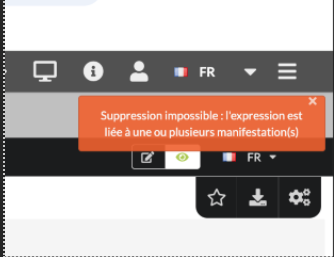
\includegraphics[width=0.7\textwidth]{images/terminologie.png} 
	
	\caption{Message de suppression d'une notice d'Oeuvre} 
	
	\label{figterminologie} 
	
\end{figure}

Cette proposition rejoint l’idée de supprimer la table œuvre cinématographique dans la gestion des masques alors que c’est la table œuvre/expression qui est couramment utilisée.  

Enfin, une confusion peut également s’installer entre les termes “œuvre liée” et “œuvre associée” dans les masques qui décrivent la manifestation par exemple. Le terme d’œuvre liée pourrait être corrigé en “œuvre parente” pour que la nature du lien soit plus claire entre les deux entités.  

\subsection{Conserver le niveau du FRBR en mode saisie sur les métas masques }

Actuellement, lors de la configuration des méta-masques, les champs glissés et déposés dans le type de notice concernée perdent la mention du niveau FRBR auquel ils appartiennent. L’utilisateur n’a plus le moyen de savoir, une fois dans la notice, que tel champ appartient à tel niveau. Conserver la mention du niveau du FRBR sur les métas masques au sein de la saisie de la notice permettrait une meilleure compréhension et visibilité pour l’utilisateur. Ainsi, par exemple, dans une notice de manifestation, le champ Titre afficherait : Œuvre – Titre.  

\section{Nouvelles fonctionnalités }

\subsection{Annotation de séquences sur un fichier vidéo numérique }

La table média actuelle permet seulement de visualiser une photo ou une vidéo, au clic sur la notice. Toutefois, il serait intéressant de développer une visionneuse spécifique à la vidéo qui permettrait non seulement de la visionner, mais également d’y placer des repères, des marqueurs, et de pouvoir l’annoter.  

Tout d’abord, deux possibilités de “séquençage” manuel seraient possibles :  

\begin{itemize}
	\item L’utilisateur saisit des repères temporels sur la vidéo sans la modifier. Ces repères sont reversés dans des champs prévus pour accueillir les “time codes” dans la notice de l’objet numérique. À l’ouverture du fichier numérique, les marqueurs laissés par l’utilisateur apparaissent, visibles sur la barre de défilement de la vidéo. L’utilisateur peut alors cliquer sur ces marqueurs pour naviguer au sein de la vidéo comme il le souhaite, et y voir les annotations associées.  
	
	\item L’utilisateur pourrait aussi vouloir segmenter le fichier vidéo en plusieurs séquences distinctes à partir de time codes précis. Dans ce cas-là, à la manière d’un logiciel de montage, l’utilisateur peut créer des cuts sur la vidéo et ainsi créer plusieurs fichiers numériques à partir de celle-ci, mais qui lui sont toujours liés. En effet, ces nouveaux objets, fragments du fichier vidéo d’origine, auraient leur propre notice de description mais resteraient rattachés à la notice principale, à la manière d’un ensemble.  
\end{itemize}

Cette nouvelle fonctionnalité permettrait d’apprécier l’hétérogénéité des collections, et s’avèrerait utile dans le cas, par exemple, de rushes documentaires non édités que l’utilisateur souhaiterait diviser par mots clés ou thématiques. La description des médias vidéo n’en serait que plus affinée et précisée.  

Par ailleurs, ce séquençage devra être effectué dans une optique d’annotation “sur” l’image, permettant ainsi d’associer des séquences plus précises à une description thématique. Concrètement, deux cas d’annotation sont possibles :  

\begin{itemize}
	\item L’utilisateur pourrait être capable de placer des tags sur des éléments de l’image (objets, personnes, éléments techniques, contenu...) et d’en décrire le contenu dans les champs prévus. La notice du média prévoit alors l’affichage d’une description par time codes, sur lesquels l’utilisateur peut cliquer pour accéder directement à l'image en question.  
	
	\item L’utilisateur peut également vouloir décrire une séquence dans sa globalité, à l’intérieur d’un time code précis. Dans ce cas, les champs sont saisis à partir d’un tag sur le time code, et non plus sur un élément précis de l’image.  L’affichage de la description dans la notice peut rester le même que le précédent.  
\end{itemize}


À l’ouverture du fichier vidéo, les annotations saisies apparaissent à droite de la visionneuse, et les times codes superposés à la barre de défilement de la vidéo.  

La description précise sur des séquences vidéo permettrait à la recherche d’être plus performante : l’utilisateur pourrait, en cherchant certains mots clés, tomber directement sur les séquences numériques associées, aux time codes correspondants. 

Il est intéressant de penser également à la mise en place d’une recherche par mots clés au sein du fichier numérique vidéo. La recherche d’un mot clé amène l’utilisateur à une séquence décrite par ce mot clé.   

\subsection{Recherche de médias par type de format  }

Il serait pratique de mettre en place, dans la table médias, une recherche par type de formats.  

L'application pourrait détecter automatiquement le format du média créé par l’utilisateur et l'indexer pour le proposer comme critère de tri/de recherche à l’utilisateur.  

Cela permettrait notamment de pouvoir rapidement visualiser les fichiers vidéo présents dans la table, au lieu de devoir faire des albums par types de médias.  

Deux types de filtres seraient pertinents à proposer :  

\begin{itemize}
	\item Type de média : vidéo, image, son 
	
	\item Format : mp4, mpeg, jpeg, mov... 
\end{itemize}

\subsection{Mise en place d’un repérage couleur pour les niveaux du FRBR }

Il serait visuellement plus intuitif d’associer une couleur à un niveau du WEMI. Ainsi, les niveaux Oeuvre, manifestation, Item auraient chacun leur couleur, et ce, dans toute l’interface de l’application :  

\begin{itemize}
\item Menu burger,  

\item Menus des notices,  

\item Méta-masques 

\item Onglets des notices 

\item Résultats de recherche 
\end{itemize}

Un repérage visuel s’opère alors pour l’utilisateur, qui peut plus facilement se repérer au sein du FRBR.  

\subsection{Mise en place d’une visualisation des liens entre entités du FRBR }

NB : Cette idée s’inspire notamment de la “balade intuitive” proposée par la bibliothèque Kandinsky dont voici un exemple :

\begin{figure}[htbp] 
	
	\centering 
	
	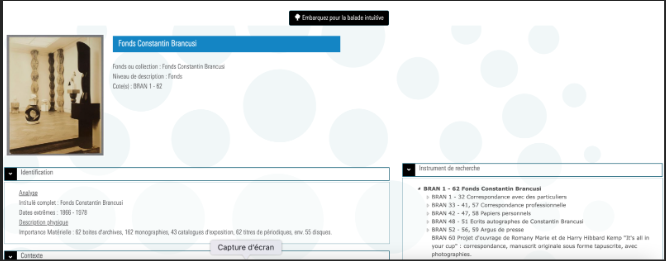
\includegraphics[width=1.0\textwidth]{images/kandinsky1.png} 
	
	\caption{Vue "balade intuitive" proposée par la bibliothèque Kandinsky \footcite{zotero-item-801}} 
	
	\label{figkandinsky1} 
	
\end{figure}

\begin{figure}[htbp] 
	
	\centering 
	
	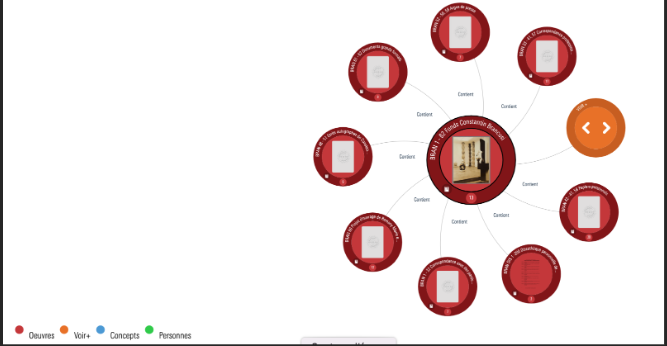
\includegraphics[width=1.0\textwidth]{images/kandinsky2.png} 
	
	\caption{Vue en graphe de la balade intuitive \footcite{zotero-item-801}} 
	
	\label{figkandinsky2} 
	
\end{figure}

Lorsque l’utilisateur ouvre S-Movies, ce sont les œuvres qui apparaissent sous la forme de résultats de recherche. Les liens avec d’autres notices (manifestations et items) n’apparaissent pas à première vue. Il faut ouvrir une notice pour voir la liste des entités qui y sont liées, si toutefois ces liens sont configurés dans le menu de la notice. Or, la visualisation de liens entre les entités d’une collection est primordiale dans la logique d’une structuration selon le modèle FRBR. Pouvoir avoir un aperçu de ces liens pourrait améliorer la compréhension de la hiérarchie entre les niveaux du FRBR et leur délimitation, et ainsi améliorer les pratiques de saisie selon les cas d’indexation. De plus, visualiser rapidement les liens entre entités permettrait d’identifier les incohérences et les erreurs de données plus facilement, comme par exemple, des éléments vides ou isolés. 

Les entités principales du FRBR étant au nombre de trois, la représentation choisie pourrait être celle d’une représentation en graphes de connaissances, modélisant ainsi les relations entre entités. Cette représentation s’appuie sur le modèle de graphe RDF (sujet-prédicat-objet) qui permet également l’interopérabilité des données.  

Pour penser la place que pourrait prendre cette visualisation des liens dans l’application, il faut se poser les questions suivantes : quel niveau du FRBR les utilisateurs préfèrent-ils visualiser ? Dans quel contexte ? Autrement dit, il faut se demander quel niveau de granularité choisir pour mettre en place cette visualisation et à quel endroit de l’application. 

Puisque la page d’accueil de l’espace de travail S-Movies présente les œuvres, la représentation en graphe pourrait dans un premier temps permettre de visualiser les œuvres présentes dans la collection.  

Le premier niveau permettrait donc à l’utilisateur de visualiser la liste des œuvres préservées sous formes de cercles, plus ou moins gros selon le nombre de sous-niveaux qu’elles contiennent. Ainsi, une œuvre qui contiendrait deux variantes, quatre manifestations, 12 items sera plus grande qu’une œuvre qui contient 1 manifestation et 1 item.  

Au clic sur l’œuvre, le détail de ses relations avec des sous-éléments apparait : variantes, manifestations, items.  

Ce mode d’affichage pourrait être disponible de la même manière que les modes d’affichage déjà présents dans l’application. Il faudrait ajouter un mode d’affichage en “graphe”. 

\begin{figure}[htbp] 
	
	\centering 
	
	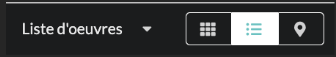
\includegraphics[width=0.6\textwidth]{images/vue.png} 
	
	\caption{Modes d'affichage disponibles dans l'application} 
	
	\label{figvues} 
	
\end{figure}

Ce mode d’affichage, établit au niveau des tables, pourrait également être disponible au niveau des notices. Par exemple dans une notice d’item, un onglet de menu pourrait être configurable pour faire apparaitre, en graphe, les relations de l’item avec les niveaux parents du FRBR.   

Il serait intéressant d’intégrer à ces visualisations en graphes les médias, d’autant plus dans le cas de la mise en place d’une segmentation vidéo, pour pouvoir visualiser les différents segments reliés à l’item.  

Concrètement, le parcours utilisateur de cet affichage serait le suivant :   
\begin{itemize}
	\item Que ce soit depuis une table ou depuis une notice, l’utilisateur clique sur le mode d’affichage en graphe  
	
	\item Les entités concernées s’affichent sous la forme de cercles, proportionnels aux nombres de liens qu’ils entretiennent avec les autres niveaux du FRBR. Les cercles comportent des informations minimales selon le niveau : le titre et la date pour les œuvres, le titre le format et la date pour les manifestations, le titre, le format, la date et l’identifiant pour l’item. 
	
	\item Une légende s’affiche en bas de l’écran avec un code couleur pour chaque entité, et le nombre d’entités présentes.  
	
	\item Au clic de l’utilisateur sur l’un des cercles, le détail des relations de l’entité avec d’autres entités s’ouvre en mode graphe. Le résumé de la notice s’affiche en barre latérale sur le côté.  
	
	\item Au clic sur une entité liée, le graphe se reforme et l’entité choisie devient le centre du graphe.  
\end{itemize}


On pourrait également ajouter au graphe les lieux et les personnes (intervenants) liés à chaque entité du FRBR. 

\subsection{Automatisation du catalogage en niveaux FRBR }

Il serait pertinent de mettre en place une automatisation de la hiérarchie FRBR à partir de la création d’une notice. Cette fonctionnalité serait assistée par l’IA. Par exemple, depuis l’item, l’application détecterait la hiérarchie supérieure à créer depuis les actions suivantes :  

\begin{itemize}
	\item Description de l’item 
	
	\item Scan du code-barres  
	
	\item Création d’une notice item depuis la table films 
	
	\item Création d’une notice item depuis la table des entrées
\end{itemize}  

L’assistant IA détecterait les liens à effectuer entre l’item en question et des notices de manifestation et d’œuvre si elles existent. Si elles n’existent pas, il créerait automatiquement les notices manifestation et œuvre et proposerait à l’utilisateur de les remplir. Ces notices seraient automatiquement liées. 

Dans le cadre de la mise en place d’un chatbot, l’utilisateur pourrait simplement décrire l’item et son contenu, et l’intelligence artificielle suggèrerait à l’utilisateur ce qu’il faut créer, ou la marche à suivre. Par exemple :  

Cet item est issu de la manifestation de telle oeuvre. Les deux notices existent déjà, il faut y lier cet item 

Cet item est issu d’une nouvelle manifestation de telle oeuvre, il faut la créer et la lier à l’item 

Cet item est issu de la variante de telle oeuvre, il faut la créer et la lier à l’item. Pas besoin de créer une manifestation, cet item est l’exemplaire unique de la variante de cette oeuvre.  


\subsection{Affichage des niveaux FRBR dans l’onglet/entête d’une notice }

Cette idée s’applique aux niveaux FRBR enfants : Variante, Manifestation, Item, puisque l’œuvre n’a pas de niveau supérieur à afficher.  

Lorsque l’utilisateur a une notice ouverte, une notice d’item-film par exemple, il n’a pas de visibilité sur les niveaux hiérarchiques parents dans lesquels s'imbrique la notice. Il serait pertinent d’afficher l’imbrication de niveaux dont fait partie la notice dans l’intitulé de son onglet.  

Actuellement, pour le niveau Œuvre, c’est le titre qui apparait dans l’onglet de la notice, tandis que c’est l’identifiant qui apparait pour la manifestation et l’item.    

À la manière d’une frise logique, l’onglet afficherait : œuvre > variante > manifestation > item. 

La notice ouverte par l’utilisateur s’afficherait en gras, pour signaler qu’elle est la notice actuellement utilisée. Dans le cadre de la mise en place d’un code couleur, les couleurs respectives de l’œuvre et de la manifestation seraient affichées dans l’onglet, en clair, tandis que le niveau appartenant à la notice ouverte serait affiché dans sa couleur, de manière vive et en gras.  

Il est important de noter que cet affichage serait plus intuitif dans le cas où les identifiants ont été paramétrés de telle sorte à pouvoir indiquer le niveau de FRBR dans l’intitulé. Par exemple : MN-0001, pour manifestation numérique 1, ou IP-0002 pour un item physique 2. Ainsi, dans l’affichage de l’onglet, cela donnerait l’intitulé suivant :  

\begin{itemize}
\item Casablanca > MN-0002 > IN-0006.
\end{itemize}  

Toutefois, même si le niveau du FRBR n’est pas indiqué dans les identifiants, l’affichage de gauche à droite induit une hiérarchie du haut vers le bas. Si un code couleur est mis en place, il pourrait rendre l’affichage intuitif sans la présence des niveaux dans les identifiants.  

Nous pouvons penser également à une modification de ce qu’affiche l’onglet de la notice pour la manifestation et pour l’item. En effet, pour que cela soit encore plus clair pour l’utilisateur, la frise présente dans l’onglet d’une notice pourrait afficher, pour la manifestation, son type. Ainsi, cela donnerait la chose suivante :  

\begin{itemize}
	\item Casablanca > pré diffusion > IP-0005.
\end{itemize}  

Même chose pour la variante :  

\begin{itemize}
	\item Casablanca > censuré > distribution en salles > IN-0007.
\end{itemize}

Notons tout de même que pour que cet affichage soit fonctionnel, la taille des onglets de notice devra être agrandie.  

\subsection{Repenser le mode de création de notices dans des tables individuelles}

La création de notices au sein de tables individuelles n’encourage pas l’utilisateur à lier les notices entre elles, sur plusieurs niveaux. Le risque est ainsi que l’utilisateur crée des notices individuelles, elles aussi, sans les relier à d’autres niveaux du FRBR. Pour éviter cela, il pourrait être intéressant de proposer, dans le menu burger, la création de liens prédéfinis, au lieu de créer au sein de tables. Les tables pourraient être alors réservées à la consultation et à l’affichage des notices créées. Cette idée rapprocherait S-Movies d’une interface où l’utilisateur crée un réseau de liens, propre à une collection cinématographique. 

L’idée serait d’ajouter un onglet dans le menu burger intitulé “Création/liens”, qui permettrait à l’utilisateur de créer des liens “préconçus”. Une sorte de création rapide, sans possibilité de créer des notices uniques.  

Sous cet onglet seraient ajoutées par exemple les options suivantes (de manière non-exhaustive) :  

\begin{itemize}
	\item Créer un item et sa manifestation 
	
	\item Créer un item, sa manifestation, et son oeuvre 
	
	\item Créer une manifestation d’une oeuvre 
	
	\item Lier un item à une manifestation
\end{itemize}
  

Au risque de surcharger l’interface, on peut également imaginer qu’au sein de chacune des tables, le bouton d’action > créer une nouvelle notice soit supprimé, et remplacé par des boutons d’action de liens. Ainsi, au lieu d’avoir une liste de propositions de liens non organisée, les propositions de liens seraient propres au lien qu’entretient chaque table avec les autres. Ainsi, par exemple : 

\begin{itemize}
	\item Table Œuvres :  
	
	\subitem Lier une oeuvre à une manifestation 
	
	\subitem Lier une oeuvre à un item 
	
	\subitem Lier une oeuvre à une variante  
	
	\item Table manifestations :  
	
	\subitem Lier une manifestation à une oeuvre 
	
	\subitem Lier une manifestation à un item 
	
	\item Table items-films :  
	
	\subitem Lier un film à une oeuvre 
	
	\subitem Lier un film à une manifestation 
\end{itemize}


Au clic, le bouton d’action propose soit à l’utilisateur de lier une entité existante à celle sélectionnée, soit d’en créer une si elle n’existe pas. Le terme “lier” dans le bouton d’action signifie ainsi également la création d’une notice en lien avec une autre, pas seulement l’ajout d’un lien entre deux notices existantes.  

La limite de cette idée est qu’elle est contre intuitive : la création d’une notice de chaque entité se fait dans d’autres tables que celle qui lui est dédiée.  

Cette refonte du mode de création des notices assure toutefois un lien indissociable entre les entités, qui permettra notamment d’empêcher la suppression d’une entité et des éléments qui lui sont liés par exemple. Cela faciliterait aussi la mise en place de visualisation des liens, si les entités sont toutes interconnectées. Surtout, ces nouvelles modalités suppriment la possibilité de créer des notices individuelles, sans lien avec les niveaux du FRBR.  